\chapter{Techno-economic analysis}

This appendix contains an approximate budget and Gantt chart for the planned activities.

\begin{table}[h!]
	\centering
	\begin{tabular}{ | m{15em} | m{3em} | m{3em} |m{4em} | m{4em} | m{4em}| } 
		\hline
		Activity & \multicolumn{2}{|c|}{Engineering time} & Running costs & Facility use & Capital costs \\ 
		\hline
		&hr & R & R & R & R\\
		\hline
		Review Literature &25&11250&250&&\\
		\hline
		Compile Design Requirements&25&11250&250&&\\
		\hline
		Design localiser device&150&67500&500&500&\\
		\hline
		Produce Prototype&125&56250&1000&1500&1500\\
		\hline
		Test Prototype&50&22500&1000&500&\\
		\hline
		Finalise Report&100&45000&500&&\\
		\hline
		Total&475&213750&3500&2500&1500\\
		\hline
		Grand Total (R)&221725&&&&\\ 
		\hline
	\end{tabular}
\caption{Estimated cost per activity}
\end{table}

\noindent This budget is based on a standard rate of R450/h. The capital costs include estimates for the microphones and Analogue to digital converter.

\begin{figure}[h]
	\centering
	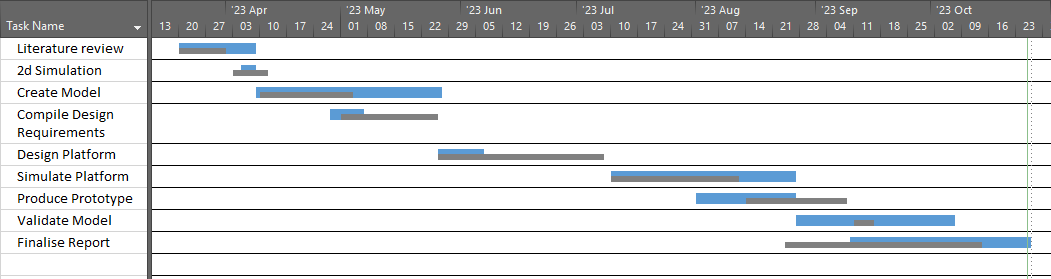
\includegraphics[width=1.5\textwidth,angle=90]{Gantt}
	\caption{Gantt Chart}
	\label{fig:mesh1}
\end{figure}